\section{logistic回归}
\subsection{梯度下降与logistic回归}
对于二分类问题,常采用logistic回归。若采用线性回归做二分类预测问题,其预测取值有可能大于1或小于0。为了解决这个问题,在$\theta^Tx$增加logistic函数变换(或称为sigmoid函数变换)
\begin{eqnarray}
h_\theta(x)=g(\theta^Tx)=\frac{1}{1+e^{-\theta^Tx}}
\end{eqnarray}
其中
\begin{eqnarray}
g(z)=\frac{1}{1+e^{-x}}
\end{eqnarray}
称为logistic函数或者sigmoid函数。其函数图像如下
\begin{center}
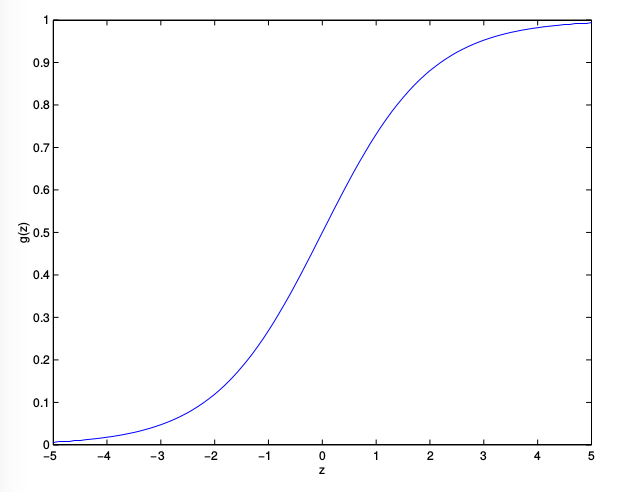
\includegraphics[scale=0.5]{../figures/cs229_2_1.png} 
\end{center}
该函数的求导结果为
\begin{eqnarray}
\begin{aligned}
g'(z) &= \frac{d}{dz}\frac{1}{1+e^{-x}}\\
&= \frac{1}{(1+e^{-z})^2}(e^{-z})\\
&= \frac{1}{1+e^{-z}}
\left(
\begin{aligned}
1-\frac{1}{(1+e^{-z})}
\end{aligned}
\right)\\
&= g(z)(1-g(z))
\end{aligned}
\end{eqnarray}
准确概率可以如下表示
\begin{eqnarray}
P(y=1|x;\theta) &=& h_\theta(x)\\
P(y=0|x;\theta) &=& 1-h_\theta(x)
\end{eqnarray}
将上式结合起来,有
\begin{eqnarray}
p(y|x;\theta)=(h_\theta(x))^y(1-h_\theta(x))^{1-y}
\end{eqnarray}
则似然函数可以表示为
\begin{eqnarray}
\begin{aligned}
L(\theta) &= p(Y|X;\theta)\\
&= \prod_{i=1}^mp(y^{(i)}|x^{(i)};\theta)\\
&= \prod_{i=1}^m(h_\theta(x^{(i)}))^{y^{(i)}}(1-h_\theta(x^{(i)}))^{1-y^{(i)}}
\end{aligned}
\end{eqnarray}
取对数似然函数,有
\begin{eqnarray}
\begin{aligned}
l(\theta) &= \log L(\theta)\\
&= \sum_{i=1}^m y^{(i)}\log h(x^{(i)})+(1-y^{(i)})\log (1-h(x^{(i)}))
\end{aligned}
\end{eqnarray}
由于其没有显式解,因而采用梯度下降法进行求解。
\begin{eqnarray}
\begin{aligned}
\frac{\partial}{\partial \theta_j}l(\theta)
&=\left(
	\begin{aligned}
	y\frac{1}{g(\theta^Tx)}-(1-y)\frac{1}{1-g(\theta^Tx)}
	\end{aligned}
	\right)\frac{\partial}{\partial\theta_j}g(\theta^Tx)\\
&=\left(
	\begin{aligned}
	y\frac{1}{g(\theta^Tx)}-(1-y)\frac{1}{1-g(\theta^Tx)}
	\end{aligned}
	\right)g(\theta^Tx)(1-g(\theta^Tx))\frac{\partial}{\partial\theta_j}\theta^Tx\\
&=(y(1-g(\theta^Tx))-(1-y)g(\theta^Tx))x_j\\
&=(y-h_\theta(x))x_j
\end{aligned}
\end{eqnarray}
则有如下更新参数的式子
\begin{eqnarray}
\theta_j:=\theta_j+\alpha(y^{(i)}-h_\theta(x^{(i)}))x_j^{(i)}
\end{eqnarray}

最后,对于给定的输入实例$x$,按照
\begin{eqnarray}
P(y=1|x;\theta)&=&h_\theta(x)\\
P(y=0|x;\theta)&=&1-h_\theta(x)
\end{eqnarray}
分别求出$P(y=0|x;\theta)$和$P(y=1|x;\theta)$,比较两个条件概率值的大小,将实例$x$分到概率值较大的那一类。
\subsection{牛顿方法}
假设有函数$f:\mathbb{R}\rightarrow\mathbb{R}$,目标是找到$\theta$,使$f(\theta)=0$,其中,$\theta\in \mathbb{R}$,其通过如下式子迭代求解
\begin{eqnarray}
\theta:=\theta-\frac{f(\theta)}{f'(\theta)}
\end{eqnarray}
迭代过程如下图所示
\begin{center}
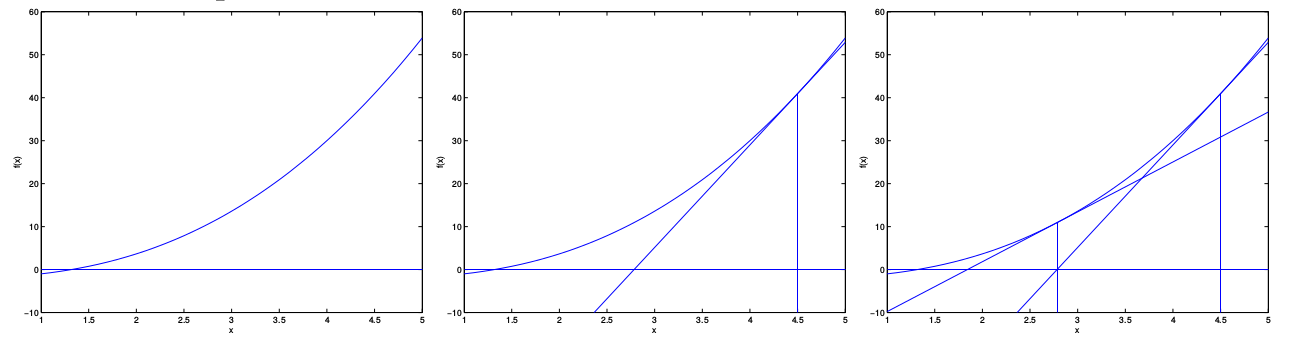
\includegraphics[scale=0.3]{../figures/cs229_2_2.png} 
\end{center}
对于logistic回归的对数似然函数
\begin{eqnarray}
\begin{aligned}
l(\theta) &= \log L(\theta)\\
&= \sum_{i=1}^m y^{(i)}\log h(x^{(i)})+(1-y^{(i)})\log (1-h(x^{(i)}))
\end{aligned}
\end{eqnarray}
考虑其最大值,即对$l(\theta)$的导数$l'(\theta)=0$进行求解,若采用牛顿方法,则有
\begin{eqnarray}
\theta:=\theta-\frac{l'(\theta)}{l''(\theta)}
\end{eqnarray}
若$\theta$为一个向量,则更新法则定义为
\begin{eqnarray}
\theta:=\theta-H^{-1}\nabla_\theta l(\theta)
\end{eqnarray}
其中,$H$为Hessian矩阵,其定义如下
\begin{eqnarray}
\begin{aligned}
H_{ij}&=\frac{\partial^2l(\theta)}{\partial\theta_i\partial\theta_j}\\
&= \frac{\partial}{\partial \theta^{(j)}}\sum_{m=1}^M(h_\theta(x_m)-y_m)x_m^{(n)}\\
&= \sum_{m=1}^M\frac{\partial h_\theta(x_m)x_m^{n}}{\partial \theta^{(j)}}\\
&= \sum_{m=1}^Mx_m^{(n)}\frac{\partial g(\theta^Tx_m)}{\partial \theta^Tx_m}\frac{\partial\theta^Tx_m}{\partial\theta^{(j)}}\\
&= \sum_{m=1}^Mx_m^{(n)}g(\theta^Tx_m)(1-g(\theta^Tx_m))x_m^{(j)}\\
&= \sum_{m=1}^Mx_m^{(n)}h_\theta(x_m)(1-h_\theta(x_m))x_m^{(j)}
\end{aligned}
\end{eqnarray}
因而
\begin{eqnarray}
\begin{aligned}
H&=\nabla_\theta^2l(\theta)\\
&= X^TRX
\end{aligned}
\end{eqnarray}
其中
\begin{eqnarray}
R=
\begin{pmatrix}
h_\theta(x_1)(1-h_\theta(x_1)) & 0 &\cdots & 0\\
0 & h_\theta(x_2)(1-h_\theta(x_2)) & \cdots & 0\\
\vdots & \vdots & \ddots & \vdots\\
0 & 0 & \cdots & h_\theta(x_m)(1-h_\theta(x_m))
\end{pmatrix}
\end{eqnarray}